\section{Software Product Lines}\label{sec:spl}
We will first give a brief introduction to \emph{Software Product Lines}.
More background details can be found in for 
example~\cite{van2001notion, apel2013software, bosch2000design}.
Software Product Lines use the same idea as age-old industrial product lines.
The idea behind them is that variants of products can be easily created when 
multiple products use the same general parts. If these parts can be created
in the same factory, we only need to combine these in different ways to create
multiple products. This idea can be read in the context of industrial
manufacturing, where we can for example create different aeroplanes that have
great overlap in their parts. We can also read this in the context of software,
this is where we talk about Software Product Lines.

Concepts used in software product lines include features, configurations,
variants and products. Since we will also use these concepts throughout this
work, let us look at them in more detail. \emph{Features} are ``\emph{a logical
unit of behaviour that is specified by a set of functional and quality
requirements}'', according to~\cite{bosch2000design}. This means that features
implement the requirements of a system, an example would be sending messages in
an e-mail system. These features can be toggled on and off, they are binary. In
source code, features can be implemented for example using \texttt{\#ifdef}
statements. \emph{Configurations} can be seen as a list of all features with
all of them either enabled or disabled. Configurations can be deemed valid with
the use of \emph{Feature Models}, which describe relations between features.
One could see how features such as \emph{Linux} and \emph{Windows} should not
occur simultaneously. \emph{Variants} or \emph{products} are configurations
applied to full systems. By applying them, certain parts in the source code can
be removed, whilst others should stay, decided by the variability mechanism
(i.e. the \texttt{\#ifdef} statements).

\begin{figure}
    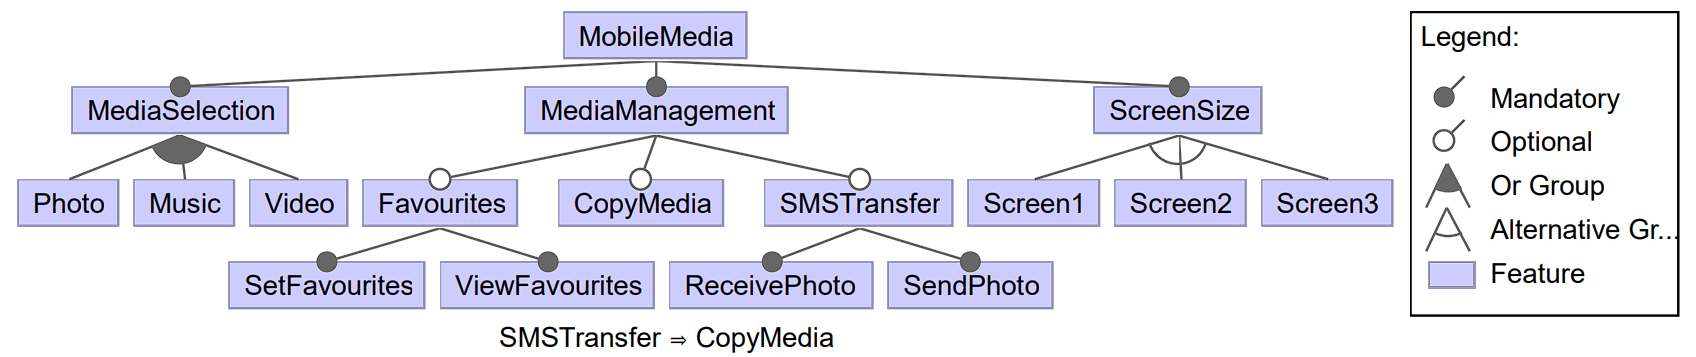
\includegraphics[width=\textwidth]{mobilemedia}
    \caption{Example Feature Model of MobileMedia}
    \label{fig:example:mobilemedia}
\end{figure}

\section{Feature Models}\label{sec:featuremodels}
Let us look at \emph{Feature Models} in more detail. As explained previously,
feature models describe relations between features. More precisely, feature
models are connected acyclic trees. The topmost feature always is a central
root feature under which other features can be placed. Growing the tree, a
hierarchy of features is created. As an example, we may have a feature
``Messaging'', which has subfeatures ``E-mail'' and ``SMS''. To be able to
create more advanced relations between features, we can place several
constraints on them. Firstly, we can define a feature to be either optional or
mandatory in relation to its parent. This would mean that (in the case of
optionality), if a parent is enabled, it is optional to enable that subfeature.
In the other case, if a parent is enabled, that child feature must also be
enabled. Of course, when we talk about something that ``must'' be the case, we
mean that the feature model is only \emph{valid} if that requirement holds.
Apart from optionality, we can also define a feature to be a \emph{group}. This
group then means that the feature designated as a group becomes the ``root'' of
that group. A group can be defined as an ``or'' group, or a ``alternative''
group. In the case of the ``or'' group, \emph{at least one} of the subfeatures of
the root of the group must be active for the feature model to hold. In
the ``alternative'' group, \emph{exactly one} of the subfeatures must be
activated.

An example feature model can be seen in Figure~\ref{fig:example:mobilemedia}.
In this feature model, we can see that the root of the model is ``MobileMedia''.
The subfeatures of this root are three mandatory features ``MediaSelection'',
``MediaManagement'' and ``ScreenSize''. The subfeatures of ``MediaSelection''
are an ``or'' group, so at least either ``Photo'', ``Music'' or ``Video'' has
to be chosen. The subfeatures of ``MediaManagement'' are optional, so they do
not have to be chosen. The subfeatures of ``ScreenSize'' are in an
``alternative'' group, which means that we need to have either ``Screen1'',
``Screen2'' or ``Screen3'', but it is limited to one of them.

We skipped over one --for us-- important detail in feature models thus far. The
example contains a boolean formula at the bottom:
\[
    \textsf{SMSTransfer} \Rightarrow \textsf{CopyMedia}
\]
These can be any boolean formula, but in this case, are limited to a simple
implication. More precisely, we would call this a ``requires'' relationship, as
the ``SMSTransfer'' feature \emph{requires} the ``CopyMedia'' feature.
These boolean formulae (there can be any number of them) must also hold, next
to the requirement of the relations defined by the tree itself. As these extra
constraints must hold for the entire tree, these boolean formulae are called
\emph{Cross-Tree Constraints}. These types of constraints will play a large
role in our research, which we will explain in more detail later.

\subsection{Extended Feature Models}\label{sec:extendedfeaturemodels}
In the introduction, we talked about feature models possibly containing 
non-functional parameters. We have seen the functional parameters in the
previous section, but have not seen non-functional parameters yet. We will
cover them here. We can include non-functional parameters in features in a
feature model, this creates a so-called
\emph{Extended Feature Model}~\cite{benavides2005extfms}. These can be
parameters such as cost and performance. We may then want to find optimal
instantiations (or products) from feature models by adding objectives to
the non-functional parameters. For example by minimising cost, or maximising
performance. Solutions are then \emph{Pareto fronts} of non-dominated
solutions~\cite{horcas2022breakit}. Finding these solutions is an NP-complete
task~\cite{ochoa2018npcomplete}, and we will go in-depth into this in the next
section.
